%\documentclass[conference]{IEEEtran}
\documentclass[10pt,twocolumn]{article}
\usepackage{timesnewp}
\usepackage{latex8}
\usepackage{graphics}
\usepackage{cite}
%\usepackage{doublespace}

\pagestyle{empty}
\begin{document}

\title{Toward A More Scalable End-User Scripting Language}
\author{%
\begin{tabular}{cc}
  \begin{tabular}{ccc}
    Alessandro Warth$^{\dag}$ &\hspace*{1cm}  &  Takashi Yamamiya$^{\dag}$\\
    {\it alex@vpri.org} &   & {\it takashi@vpri.org}\\
\\
    Yoshiki Ohshima$^{\dag}$  & & Scott Wallace$^{\dag}$\\
    {\it yoshiki@vpri.org} & & {\it scott@vpri.org}
  \end{tabular}\\
\\
\end{tabular}\\
\begin{tabular}{c}
$^{\dag}${\it Viewpoints Research Institute}\\
{\it 1209 Grand Central Ave.}\\
{\it Glendale, CA 91201}\\
\end{tabular}
}

\maketitle\thispagestyle{empty}

\renewcommand{\thefootnote}{\fnsymbol{footnote}}%
\footnote[0]{This material is based upon work supported by the National Science
Foundation under Grant No. 0639876.
Any opinions, findings, and conclusions or recommendations expressed
in this material are those of the author(s) and do not necessarily
reflect the views of the National Science Foundation.}%
\begin{abstract}
End-user scripting languages are relatively easy to learn, but have
limited expressive power.  Tile-based scripting systems are
particularly accessible to beginners, but usually are very limited in
scope and usually lack extensibility, and for some tasks the tile
idiom becomes cumbersome.  Conventional programming languages used by
computer professionals are far more powerful, but at the cost of
additional complexity and limited environmental support, which place
them out of the casual programmer's reach.  This paper presents
TileScript, an attempt to combine the accessibility of a tile-based
programming interface with the leverage of a full textual programming
language and with a simple means of extension, making it potentially
an appealing tool for the novice programmer without sacrificing any
expressiveness.  All TileScript programs, whether built originally
with tiles or textually, can always be edited both graphically via a
drag-and-drop tile interface and textually, and the user can freely
switch back and forth between tile and textual representations at any
time.  Additionally, TileScript's simple yet powerful extensibility
mechanisms allow the language to be used to tackle problems that would
normally be out of the scope of an end-user scripting language.
\end{abstract}


\Section{Introduction}

Computers are present in virtually every aspect of our lives:
middle-schoolers and grandmothers alike use them at home, at school,
and at work. Sadly, computers are mostly used for activities like word
processing, web browsing, e-mail, and games. To truly take advantage
the power of their computers, {\em end-users} must be able to write
programs. This makes end-user programming languages and environments
an important area of research.

A number of end-user programing systems have been proposed.
These systems have focused on various goals, and can be
classified based on several criteria.  One such criterion is the {\em
steepness of the learning curve} --- in other words, how easy it is for
a new user to become productive.  In systems like
Viscuit~\cite{yh03viscuit} and StageCast~\cite{dcs00stagecast}, for
example, simple graphical pattern-matching and rewrite rules allow
end-users to compose simple animations quickly and easily, with very
little training required.

Another criterion is the {\em ceiling height}, i.e., how well the language scales to more complex
problems. A full-fledged programming language with many built-in
features, where the user writes textual programs, will get the highest
marks on this criterion.

  The tension between these criteria makes the task of designing an end-user
programming system a difficult one.
No system that we are aware of has both a gentle
learning curve {\em and} a high ceiling.  Existing systems tend to
spread on the spectrum from gentle learning curve/low ceiling to
steep learning curve/high ceiling.  Viscuit, for example, has a
very low learning curve, but expressions in Viscuit are represented
solely iconically; Viscuit, in fact, does not even have the concept of
numbers or arithmetic.  In such systems, one quickly hits the rather
low ceiling, after initially enjoying simple and easy programs.

  Systems like Scratch~\cite{mbkrsr04@scratch} offer graphical building blocks
that the user can manipulate and combine
with the mouse to construct programs.  The blocks are symbolic
representations of the elements of a program (such as numbers, symbols, and control structures) so the user
has to learn what each block does and means, but as he learns more
about these blocks, his productivity increases.
Unfortunately, this gentle learning curve has some negative
consequences; for example, Scratch intentionally omits the concept of inter-object
reference to avoid confusion.  This design choice makes it
tricky to write a program where multiple objects work together.

  At the other end of the spectrum, there are languages and systems
with fully textual code.  Many educational and end-user development
environments are based on Java, Python and other conventional
languages, which makes them very expressive.  Also, text-based
programming tends to be more efficient than tiles as programs grow in complexity.
{\em Processing}~\cite{rf07processing} and J0~\cite{j0} are based on
simplified versions of Java, and provide end-user-oriented
development environments.  However, users have to deal with syntax
errors, and face a steeper learning curve.

\begin{figure}[tp]
\centering
\scalebox{0.4}{\includegraphics{turtle.eps}}
\caption{A screenshot from the TileScript system.  The smae code is shown as tiles and text-based code.}
\label{fig:turtles}
\end{figure}

\SubSection{The Goal}
  Our goal is to create a new end-user scripting language with a gentle learning
curve and a high ceiling.  Our system should support both tile scripting and
textual coding, and the transition between these two representations should be as
smooth as possible.  Specifically, we aim to make it possible for the user to:
\begin{itemize}
\item
  convert a tile script into equivalent textual code, and vice-versa;
\item
  extend the system by creating new kinds of tiles (abstractions), and optionally customize
  their appearance. (The meaning of new tiles should be described using
  tiles or textual code.)
\item
  ``pop the hood'' of any part of the system, so that he can learn about (and perhaps even modify) it.
\end{itemize}
Although users will most likely get started using the tile scripting interface, all
of the
knowledge they acquire with the tiles will still be valid
once they make the transition to text-based programming.

  Our idea draws upon Squeak
Etoys~\cite{ack97Etoys}\cite{bjkr03PowerfulIdeas}.  Etoys, like Scratch,
offers visual building blocks (called ``tiles'') which the user can
combine by dragging-and-dropping to make a unit of program called
a {\em script}.

\begin{figure}[tp]
\centering
\scalebox{0.4}{\includegraphics{etoystiles.eps}}
\caption{The same Etoys script in graphical representation and textual representation.}
\label{fig:etoys tiles}
\end{figure}

Etoys tile scripts can be converted into textual code (represented in the system's base language,
Squeak Smalltalk), as shown in Figure~\ref{fig:etoys tiles}.
Unfortunately, this conversion
is only ``one way''; once the user edits the code
textually, there is no mechanism to convert the edited text back to
tiles.
This limitation exists because Smalltalk is a lot more expressive than the tile language, which
makes it is possible for the user to type in code that does not have a
corresponding graphical tile representation.
Also, the Etoys object model is not the same as Smalltalk's, which means that 
the knowledge of the model the user acquires by using Etoys cannot be
translated to Smalltalk programming.
Lastly, because Etoys tiles are implemented in Smalltalk by the system's developers, the end-user is
cannot extend the tile language with new tiles; he is limited to using the ones provided by the
developers.

\begin{figure}[tp]
\centering
\scalebox{0.7}{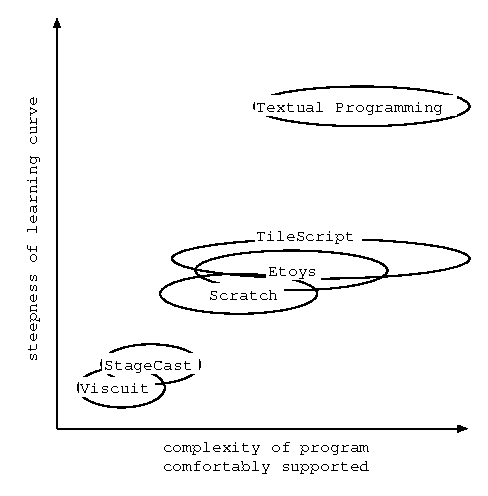
\includegraphics{spectrum.eps}}
\caption{A classification of various end-user programming systems.}
\label{fig:spectrum}
\end{figure}

%% \SubSection{Problems for Providing Extensibility and Openness}

%%   There is another axis in our classification of end-user programming
%% systems; it is {\em extensibility} of the system.  Most of the
%% end-user systems typically provide pre-made, fixed features (such as
%% the matching rules in Viscuit and StageCast, blocks and tiles in
%% Scratch and Etoys, or the Java API in Java).  The Etoys system lets
%% the user create a new script, and the script can be used as a command
%% tile similar to the built-in ones.  However, this is as far as the user
%% can go; the code behind creation of a script is written in Smalltalk
%% by developers who have deep knowledge of the structure of classes.

%%   In visual pattern-matching languages, it is not even conceivable
%% for the user to define new kinds of matching rules.  In the environment
%% for a textually-coded programming language, adding a method or defining
%% a class (for example) is easy, but the system is not usually opened to
%% the end-user, so that defining a new control structure, for example. is usually not
%% possible.

%%   For better educational value, we contend that the entire system
%% should be at least visible to the user.  And it is also desirable that
%% the user be allowed to modify the system, based on an easy to understand model.
%% This almost implies that the entire system should be made of the same
%% thing, and that on top of it we should simply provide good interfaces suited to various end-users for various purposes.
  Figure \ref{fig:spectrum} shows a comparison of the systems described in this section.
In the figure, the vertical axis
denotes the steepness of learning curve; the lower the oval is located,
the easier to start using.  The horizontal axis denotes the complexity
of programs one can write {\em comfortably} in the system.  Our proposed 
system in the middle has similar steepness of learning curve as
Etoys but trys to cover wider kind of programs.

\SubSection{Approach}

  We chose to use JavaScript~\cite{ecma99javascript} as the basis for {\em TileScript} both because
of its simple object model and good reflective facilities, and because we had already produced our own
implementation in Squeak.

  Building our system on top of Squeak gave us access to the Morphic graphics
framework~\cite{jm02MorphicNuBlue}, which facilitated the creation of our tile-based
user interface and gave us access to a rich library of graphical objects.

  We extended our JavaScript implementation with a simple macro system.
TileScript's user-defined tiles are implemented as macros; since
macros are also part of our base language, they can be written using
tiles as well as textual code.

  TileScript programs are stored as parse trees.
We implemented conversions from textual code and tiles to parse trees,
and from parse trees to textual code and tiles.
Thus, tiles and textual code are views of the same model.

  Lastly, we provided a mechanism that allows users to customize the
visual appearance of new as well as existing tiles.

  Figure~\ref{fig:turtles} shows a screenshot from the system.  The
function that draws a triangle is shown in tiles on the right and in
text at the bottom in a JavaScript object inspector.

  The rest of this paper is organized as follows.  Section~\ref{sec:js}
briefly describes our JavaScript implementation and our extensions to the language.
Section~\ref{sec:tile implementation} describes our extensible tile-based programming interface.
In section \ref{sec:discussion}, we discuss the findings from
this experiment.
Section~\ref{sec:related} discusses related work.
Section~\ref{sec:conclusions} discusses future work and concludes.

\Section{Our JavaScript Implementation}
\label{sec:js}

  JavaScript is a language that features a dynamic, prototype-based object
model.  It has notably rich reflective features.  While existing
implementations widely used in common web-browsers and elsewhere
provide these dynamic and reflective features, we decided to implement
our own JavaScript on top of Squeak, which is another
dynamic language.  This approach allows us to change the
language freely, to do deeper introspection of program execution, and
to leverage the powerful Morphic GUI framework.

  To capture the syntax structure of code, we have added a new macro
system to the language.  We use macros as the internal
representation of tiles in our tile-scripting system.  Since macro definitions are
made in the same language, the end-user can write his own macros and hence define his own tiles, as we shall see below.

  In the rest of this section, we briefly explain our base implementation of
JavaScript and the macro system.

\SubSection{The Base Implementation}

  Our JavaScript parser and compiler are written in OMeta~\cite{wp07ometa}.
%  OMeta is inspired by
%Packrat parser~\cite{b02packrat} but it also provides multi-level
%pattern matching features typically found in functional languages in
%seamless manner.
OMeta programs resemble EBNF grammars with interleaved
semantic actions;
we use a few different OMeta grammars to
convert JavaScript programs to executable Smalltalk code.

  A JavaScript object is a dictionary-like entity, so it is
represented as a {\sf Dictionary} in Squeak.  JavaScript field accesses
are converted to Squeak dictionary access-by-key operations, with
delegation to the prototype object.

  Our JavaScript implementation is written in $350$ lines of OMeta, together with
$750$ lines of JavaScript library code written in JavaScript itself.  This
compactness is one of the keys in this project, as we would like to
make the inner workings of our system fully accessible to the user.

\SubSection{The Macro System for Tiles}
\label{ssec:macro system}

\begin{figure}[tp]
\begin{quote}
\hspace*{0mm}\verb+macro @if(cond, tbranch, fbranch) {+\\
\hspace*{5mm}\verb+if (cond)+\\
\hspace*{10mm}\verb+tbranch+\\
\hspace*{5mm}\verb+else+\\
\hspace*{10mm}\verb+fbranch+\\
\hspace*{0mm}\verb+}+\\
\end{quote}
\caption{Definition of the {\tt if} macro.}
\label{fig:macro if}
\end{figure}

We have added a macro system to the base implementation described above.
A macro definition begins with the {\tt macro} keyword, followed by a macro name,
which must start with a {\tt @}.
For example, Figure~\ref{fig:macro if} shows a macro version of the {\tt if-then-else} statement,
which can be used as follows:

\smallskip
\noindent\verb+@if(5 > 6, alert("yes"), alert("no"))+
\smallskip

\begin{figure}[tp]
\begin{quote}
\hspace*{0mm}\verb+macro @repeat(k, body) {+\\
\hspace*{5mm}\verb+var n = k+\\
\hspace*{5mm}\verb+while (n-- > 0)+\\
\hspace*{10mm}\verb+body+\\
\hspace*{0mm}\verb+}+\\
\end{quote}
\caption{Definition of the {\tt @repeat} macro.}
\label{fig:macro repeat}
\end{figure}

%  The arguments to the @-macro (in this example, {\tt alert("yes")}
%and {\tt alert("no")}) are written in the same language and parsed in
%the same parser, and the converted sub parse trees are embedded in the
%macro definition written in the same language.

  The example we are going to use in the rest of this paper is the {\tt
repeat} statement.  Repeat is a simplified version of the {\tt while} loop
that is useful in turtle geometry and other end-user oriented
programs.  The macro definition of {\tt repeat} is given in Figure~\ref{fig:macro repeat}.
Note that upon expansion, the local variable {\tt n}
will get a unique internal name so that nested {\tt repeats} will work.

  Macro expansion happens at compile time, whereas at parse time, macro
applications are kept in the parse tree; a macro instantiation
corresponds to a tile instance, and the conversion from/to the
graphical tile is done to/from the parse node that represents the
macro instantiation.  For example, when the user writes a code snippet
with the macro, like:
\begin{quote}
{\tt @repeat(10, alert("hello"))}
\end{quote}
a {\tt repeat} object is created and its two fields are initialized
with the arguments (i.e., a parse tree for {\em 10} and another parse tree for
{\tt alert("hello")}).

  Notice that the bodies of the macros in our system are written in the end-user language,
which simplifies the task of creating a new tile.

%% \begin{figure}[th]
%% \begin{center}
%% \begin{verbatim}
%% primExprHd ::=
%%         <tok '('> <expr>:e <tok ')'> => [e]
%% |       <tok #name>:n                => [{#get. #ctxt. {#quote. n}}]
%% |       <tok #number>:n              => [{#quote. n}]
%% ...
%% \end{verbatim}
%% \end{center}
%% \caption{A portion of our JavaScript parser}
%% \label{fig:js expression}
%% \end{figure}


%%   Figure \ref{fig:js expression} shows a portion of
%% the parser description.  The left-hand side of {\tt ::=} specifies the
%% production name ({\tt primExprHd} in the figure) and the right-hand side
%% specifies the choices delimited by {\tt |}.  The right hand side may contain other productions and non-terminals,
%% and on the right-hand side of the {\tt =$>$} operator, the end result is returned as a Smalltalk
%% Array created by the Squeak array constructor (enclosed by curly
%% braces).  In another part of the definition, say the {\tt number}, the
%% terminal symbol is specified by a string {\tt ''} or character and the
%% parser tests whether the input stream at the current position matches it.


\Section{Tile Implementation}
\label{sec:tile implementation}

  The macro system described in the previous section allows us to make any desired subset of a textual
language available for viewing in graphical form.  The textual code is
parsed to create a parse tree.  In this section, we describe the conversion to
graphical tiles from the parse tree, as well as conversion in the opposite direction.

\SubSection{Conversion To Graphical Tiles}
For each macro application, the parser creates an instance of the JavaScript
``class'' {\tt Tile} that represents a node in the parse tree.
There are different kinds of {\tt Tile} objects to represent different
types of syntax nodes; we provide pre-made {\tt Tiles} for each basic JavaScript construct such as {\tt
if}, {\tt while}, etc. so that these
can be also represented visually.  These different {\tt Tiles}
delegate to a ``superclass'' called {\tt GenericTile}, which
defines common behavior for all tiles; the specific tile types 
specialize this inherited behavior as appropriate.

  A method called {\tt makeTile()} is implemented by the {\tt Tile}s.
In the TileScript implementation, this method escapes to underlying
Smalltalk code that creates the graphical tile representation in the
Morphic GUI framework.  Since the tiles can be nested, {\tt
makeTile()} is also called recursively to create nested graphical
tiles.

\begin{figure}[tp]
\centering
\scalebox{0.4}{\includegraphics{hypowhile.eps}}
\caption{The appearance of {\tt while} statement with default look.}
\label{fig:hypo while}
\end{figure}

\begin{figure}[tp]
\centering
\scalebox{0.4}{\includegraphics{realwhile.eps}}
\caption{The appearance of {\tt while} statement with customized look.}
\label{fig:real while}
\end{figure}

  We could have used a single, universal, graphical
representation for every macro, since all macros
have the same structure (i.e., one parent and zero or more children
nodes.)  Figure \ref{fig:hypo while} shows a hypothetical visual of the
{\tt while} statement in this generic way.  The generic tile would be
created with a list of sub-tiles, which would then be laid out in a simple
manner.

  However, we would like to provide better looking, better-suited, and more distinctive, tiles for the
most commonly used basic language constructs.  For example, the graphical
representation of {\tt while} actually looks like Figure \ref{fig:real
while}.  

  The specialized look of such a tile is created by hand in Morphic.
Morphic provides a direct manipulation interface for creating and
copying ``Morphs'' (``Morph'' is the basic graphic object in Morphic), for changing
their size, color, border, etc., and most notably for embedding them into
one another.  By using this interface, we manually create a Morph structure
that serves as the ``template'' for a particular tile.

  The tile designer may embed as many ``spacer'' Morphs, and other cosmetic Morphs, as he wishes, to lay
things out nicely and to create precisely the appearance he prefers.  He then needs to designate (via a menu) a morph to represent each ``hole'' to be
filled by tiles dropped by the user during drag-and-drop tile scripting; each  ``hole' Morph'' is subsequently marked with a distinctive Morphic  ``property'' so that the TileScript
system can know which morphs are to be replaced.  In the case of {\tt while}, for example, there are two holes' to be marked, one for the boolean expression to be evaluated, and another for the statement(s) to be repeatedly executed.

  In the implementation of {\tt makeTile()} for a tile which has such a user-defined
graphical tile template, the template is deeply copied and then
the Morphs that represent the holes are replaced by the tiles that represent
sub-trees.

  The end-user can easily use the same mechanism to create customized tiles to suit his personal taste.  For {\tt repeat}, for
example, the end-user would assemble Morphs and make a good-looking
Morph with (more than) two submorphs.  He would then identify two
morphs (the iteration count and the body) via the UI.  Once the user
is happy with the look, TileScript stores the Morph as the new
template for {\tt repeat}.

  Note that it is not strictly necessary to create a customized look for
a user-defined tile; the generic tile can provide the same editing
functionality.

  When a macro node in the parse tree contains a non-macro (i.e.,
textual) node, a special kind of tile that behaves as a text field is
instantiated.  The layout algorithm of these tiles (including the text
field tile) is simple at this point and resulting morphs tend to be
sparse when the user mixes textual code and tiles.

  Needless to say, the tile representation can be edited graphically.
The user may obtain new tiles from any of the available
templates, drag-and-drop them to construct a function, or delete
tiles by dragging them out of structure, and he can type in expressions in the text
fields.

  Each of the basic constructs in textual code (such as {\tt
while}, {\tt if}, or a function application), has its own pre-defined macro.

\SubSection{Conversion from Graphical Tiles}

  So far we have explained how to create a graphical representation from
textual code that contains macros.  To enable graphical
editing by the user, we also need a way to convert the
graphical representation back to a parse tree and to textual code.

  If we look at a graphical tile (represented as a Morph) in the
script, there are submorphs that are marked as particular sub-nodes in
a tree.  The converter recursively looks at the sub trees in the
Morph and converts them to parse trees.

  For a user-defined tile, the same macro definition can be used to do
the conversion from tiles to the macro node.  The macro specifies the
name of tile, and the names (and numbers) of arguments.  As long as
the user marks the morphs that represent the sub-trees (provided as
arguments) properly, the converter can visit the submorphs and convert
them to partial parse nodes.  Then, the parse node object for the user-defined tile itself
is created with these sub-trees.

  Each parse node knows how to convert itself to textual code, which makes it possible for
parse trees to be rendered as text.  In the current
implementation, the indentation and layout in the original text is
lost even if the user were only to write some textual code, convert it to the
tiles, and then go back to textual code without modifying the tiles; we are
planning to add more attributes to parse tree nodes so that
properties such as comments, indentation levels, and positions in the
original source code are preserved when possible.

\SubSection{Conversion from Base JavaScript to Macros}
  It is also useful to be able to convert arbitrary textual code written in the
base JavaScript language (i.e., without macros) to the form with macros.  To do
this, we provide a macro definition for every JavaScript construct.
The definition of {\tt @if} above is an example of such a macro.  By
running a visitor that converts JavaScript constructs to macros,
one can convert the textual JavaScript code to tiles.

%\Section{Execution}
\label{sec:execution}

  In the previous section, we provide an example to add a new kind of
tile called {\tt repeat} to the language.  However, how is the
semantics of it described?

  The macro for {\tt repeat} defines a new JavaScript object that is
used to represent the node in the parse tree.  For example, when the user
writes a code snippet with the macro as:
\begin{quote}
{\tt @repeat(10, alert("hello"))}
\end{quote}
, a {\tt repeat} object is created and its two fields are initialized
with these arguments (a parse tree for 10 and another parse tree for
{\tt alert("hello")}).

  As shown in Figure \ref{fig:macro repeat}, the macro specifies the
semantics, but the we would like to make it accessible to the
end-user.  Because the definition in Figure \ref{fig:macro repeat} is
in the same language, we can re-use the same GUI ``scriptor'' widget
for defining the expanded form.




%%   The semantics definition for this is done by writing a method called
%% {\tt eval()} in the same language.  For {\tt Repeat} case, the use
%% would write the {\tt eval()} method as follows.
%% \begin{figure}[th]
%% \begin{center}
%% \begin{verbatim}
%% Repeat.prototype.eval = function(ctxt) {
%%    var i = this.n(ctxt).eval(ctxt)
%%    while (i > 0) {
%%       i = i - 1
%%       body(ctxt).eval(ctxt)
%%    }
%% }
%% \end{verbatim}
%% \end{center}
%% \end{figure}

%% As you see, {\tt eval()} function recursively calls other elements'
%% {\tt eval()}.  The {\tt ctxt} argument is the dynamic execution
%% context so that if there is a variable reference in {\tt body}, it can
%% correctly look up the value.

%%   So far, it seems relatively simple. But our goal is not only provide
%% an easy way to define a new tile, but also ``isomorphic'' projection
%% of the tile language and textual language.  Each language element,
%% including {\tt while} used above, field access, and a method
%% definition have to have the tile representation.

%%   This means that for the {\tt while} syntax, we define {\tt While}
%% object and {\tt eval()} method, and for the {\tt function} syntax to
%% define a new function, we define {\tt Function} object and {\tt
%% eval()}.  In these {\tt eval()}s, we cannot use what we are
%% defining otherwise the meta-circularity doesn't terminate.

%% \begin{table}[th]
%% \caption{Primitives}
%% \label{tab:primitives}

%% \begin{tabular}{l|l}
%% \end{tabular}
%% \end{table}

%%   For this reason, we provide a 0-level construct for certain
%% primitive language construct.  Table \ref{tab:primitives} shows the
%% such primitives.  The {\tt eval()} for these primitives are also
%% written in JavaScript; but they are not the same thing.  (How?)


\Section{Discussion}
\label{sec:discussion}

  In this section, we discuss our findings and prospects for future work.

\SubSection{Extensibility}

  One of our goals was to provide fully bi-directional transformations
between textually-written code and graphical tiles.  We succeeded in doing this.  However,
we feel that our
implementation is not as deeply extensible as it should be,
for we can neither view nor modify the
semantics and syntax of the language itself.

  We had attempted to define a method called {\tt eval()} in
JavaScript for each kind of parse node; i.e, we tried to provide a
meta-circular implementation of JavaScript which
could be viewed and modified in the same system.  However, a
meta-circular definition has to have a fixed point, and we realized
that the fixed point cannot be so {\em deep}; a function definition
requires functions defined, a function call uses many function calls,
getters and setters get and set values from objects, and {\tt if}
requires a {\tt if} statement.  These facilities cannot be written in
the user-level language.  In the other words, they have to be
``primitives'' and the user cannot modify them, for example, using tiles.

  In this sense, we contend that the macro system provides better
separation between the base language and the language that the
end-user works with.  For example, consider the {\tt @if} macro.  The user can
still change the look of its associated tile, and even change its semantics.
From the user's point
of view, this is a very powerful concept even though he can neither
change nor even see the definition of {\tt if} in the base language,

  We would like to revisit this issue in the future and try to
define a language with a smaller core.

\SubSection{The Choice of Base Language}

The choices of base language and end-user language have interesting
trade-offs.  Having a mainstream syntax helps to lower the
learning curve in a practical sense, but from the standpoint of
making text and tiles isomorphic, it can be problematical.

For instance, we would like to provide a model of the grammar that advanced end-users
can access and understand.  One of the authors made a kind of a visual
grammar editor called LanguageGame~\cite{ty03languagegame}.  We plan
to experiment with an end-user grammar editor along the line of
LanguageGame.

Had we decided to use a language with uniform syntax, like LISP or Scheme,
as our base language, it would be fairly easy for end-users to understand the
grammar, because it would be so simple.
Javascript syntax has a much more complex grammar, and will certainly make
the addition of extensible syntax to our system more difficult on the end-user.

\SubSection{The Type System}
  One of the biggest advantages of tile scripting is that it can be
made type-safe without any additional complexity.
The drag-and-drop interface can be made so that only
type-conforming tiles may be combined, and the resulting script
doesn't produce any run time errors.

  TileScript does not currently have any type-checking mechanisms.
Since TileScript allows textual coding and conversion to tiles, developing a
reasonable type system will be an interesting challenge.

\SubSection{Formatting Textual Code}

  In the current implementation, parse tree nodes do not carry any
information about the formatting of their corresponding textual code.  Consider what happens when the user writes
some code textually, converts it to tiles, and then makes some very small
modification.  If he converts the tiles back to textual code, all
formatting information such as indentation and line breaks will be lost.
In order to minimize such nasty surprises, TileScript parse tree nodes should contain as much formatting
information as possible (these should be stored as properties), and the different conversions
take them into account.

\SubSection{Structure of Tiles}
  In our current implementation, the visual appearance of a tile
script follows the structure of the parse tree.  This is fine in most of the
cases, but can be cumbersome for a chain of arithmetic operators.  For
example, if the user thinks about an expression:
\begin{center}
{\tt sum = a + b + c + d + e}
\end{center}
he does not need to think about operator precedence; it is better
to simply think of the above expression as the ``sum of five values''.
However, the in the tile representation, the user is inevitably forced
to look at nested expressions as shown in Figure~\ref{fig:nested
tiles}.  A sophisticated tile scripting environment should allow the
user to edit such expressions in less rigid ways.

\begin{figure}[tp]
\centering
\scalebox{0.5}{\includegraphics{sum.eps}}
\caption{A nested tree from a flat expression.}
\label{fig:nested tiles}
\end{figure}


\Section{Related Work}
\label{sec:related}

Scratch is a tile-based scripting language for kids. A pervasive simplicity and a well-polished user interface make Scratch a welcoming environment for first-time users.
Naturally, this ease of use comes at a price.  Unlike most other programming languages, Scratch
provides no form of abstraction (e.g., users cannot create their own tiles or functions.) Scratch projects that go beyond a certain threshold of
sophistication tend to contain unwieldy programs that can be difficult to write and to maintain.

%Scratch is a tile-based scripting language for kids. Unlike most other programming languages, Scratch
%does not support any form of abstraction (e.g., users cannot create their own tiles or functions); this level of
%simplicity, combined with a well-polished user interface, makes Scratch a welcoming environment for first-time users.
%Unfortunately, this ease of use comes at a high price: Scratch projects that go beyond a certain threshold of
%sophistication tend to contain unwieldy programs that are frustrating to write and to maintain.

Our own Squeak Etoys, another easy-to-learn tile-based scripting language, supports user-defined
procedures, or {\em scripts}. Although Etoys scripts cannot return values (which makes them less powerful than
functions), they provide an important form of abstraction that in turn enables users to tackle moderately
sophisticated projects without ``feeling like a dog standing on its hind legs''. This is clearly a step in
the right direction, but we can do better.

TileScript is our attempt to create an end-user programming language that is just as welcoming to new programmers as
Scratch and Etoys, but which scales to arbitrarily complex tasks like a conventional programming language.

Squeak's Universal Tiles (UniTiles) was an earlier attempt at creating a more scalable end-user scripting system.
UniTiles was isomorphic to Smalltalk, which made it just as expressive as---but no easier to
learn than---Smalltalk. Additionally, because Smalltalk does not support macros, a UniTiles implementation of our {\tt
repeat} example would require its {\tt body} argument to be passed in as a block, which can be confusing to beginners.
TileScript's macro construct and its associated user interface component make it easy for end-users to define their own
control structures.

Like TileScript, IMP~\cite{i70imp} allowed programmers to define their own control structures using a macro-like mechanism.
The main difference between these two approaches is that IMP was based on syntax extension: each new control structure
was accompanied by a BNF description of its intended syntax. The analog of syntax extension in TileScript is our
tile-creation GUI, which allows end-users to design the look-and-feel of the tile associated with a particular macro. We
believe this approach to provide a better fit with our intended users, who are not expert programmers.

\Section{Conclusions}
\label{sec:conclusions}

  In this experiment, we added a small macro system to JavaScript to
capture both the syntactic structure and the semantics of textual code into parse tree nodes that are
used as internal representations of the code.
We also described conversions between arbitrary tile scripts and arbitrary textual code, which work in either direction.

  With these facilities, we managed to build a system in which
new kinds of tiles in the tile-scripting system can be defined in a way accessible to end-users.
  All of the constructs of our language are available to the end-user in both tiles
and text, which allows the end-user to explore all aspects of the system in a fairly deep manner.

  This project is still in its infancy.  As discussed in the previous
section, we aim to allow even deeper exploration by defining more parts
of the system in itself, and also to make the system more practical for
real end-users to use effectively.

\section*{Acknowledgement} We would like to express thanks for the
  valuable insights that Alan Kay, Kim Rose, Ted Kaehler, Bert
Freudenberg, Ian Piumarta, and other colleagues have given us.



\bibliographystyle{IEEEtran}
\bibliography{sts}
\end{document}

%% for i in *.png
%% do
%%    "c:/Program Files/ImageMagick-6.0.1-Q16"/convert $i `basename $i .png`.eps
%% done
